\section{La gamification comme motivation}
\subsection{Expérience de "sensing"}
La première amélioration attendue après gamification est l'amélioration de la motivation et de l'implication des participants. Dans le cadre d'une activité de "participatory sensing" réalisée via une application mobile~\cite{gamif-partici},  les participants vont relever diverses informations à des endroits qui leur sont indiqués, par exemple les conditions météorologiques et la fluidité du trafic routier à un croisement de rue donné. L'expérience réalisée ici récompensait par de petites sommes d'argent les participants pour chaque tâche effectuée, sommes augmentant selon la distance parcourue et la tâche effectuée. L'expérience consistait à rajouter un système de badges, de classement et de prix pour les tâches plus complexes afin de motiver davantage les utilisateurs sans augmenter les sommes à verser.\par

Les participants ont été répartis dans trois groupes, ou clusters, en plus d'un groupe témoin :
\begin{itemize}
    \item Le premier cluster sépare les utilisateurs par niveaux, augmentant selon l'expérience obtenue via les tâches réalisées
    \item Le deuxième utilise un système de score augmentant avec le nombre de tâches réalisées et leur complexité
    \item Le troisième distribue des badges au participants sans système de classement
    \item Enfin, le groupe témoin utilise le système de base de l'application, à savoir un système de points marqués en fonction des tâches, échangeable contre des sommes d'argent
\end{itemize} \par

Les tâches sont réalisés grâce à la géolocalisation des utilisateurs. Elles consistent à aller jusqu’à un endroit indiqué par l’application et à valider  le déplacement au point marqué sur la carte. Les points ou badges indiqués dans la définition de la tâche sont ensuite attribués. Le déplacement vers ces points d’intérêt permet de recueillir les données de l’environnement parcouru par les utilisateurs.

\subsection{Impact sur la participation}
Là où le groupe témoin présente une participation de 53\% au tâches proposées, avec motivation financière à la clé, la mise en place de la gamification la fait passer à 73\%. On remarque que la mise en place de niveau d'expérience, qui en plus de monter au fur et à mesure récompensent avec davantage de points lorsque plus élevé, entraîne une augmentation de la probabilité de participation~\ref{fig:rewards}. Bien que le gain en point soit plus faible au démarrage, la participation augmente globalement avec la montée de niveau, et par conséquent avec l'augmentation de la gratification. \par

Les dix-huit participants à cette expérimentation ont tous montré une meilleure implication dans la collecte d'informations. Quand questionnés sur la raison principale, selon eux, de cette participation, la majeure partie a répondu que le fait que tout le monde participait et qu'ils voulaient atteindre des niveaux plus élevés étaient les facteurs les plus motivant. \par

Les auteurs envisagent de réitérer une expérience similaire dans le futur afin d'observer l'impact plus précis des points marqués durant la participation, ainsi que la présence d'une limite dans le temps pour réaliser la tâche, ainsi qu'en utilisant un échantillon de participants plus grand.


\begin{figure}
    \centering
    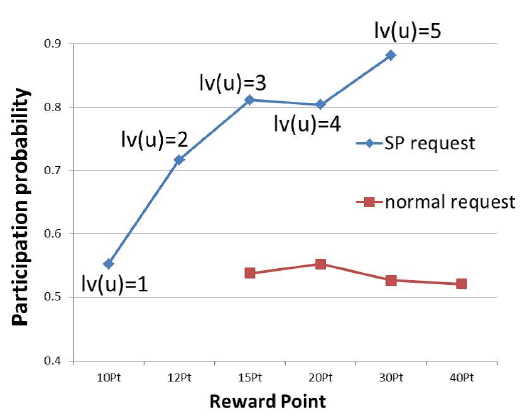
\includegraphics[width=0.7\linewidth]{Images/sensing-participation-figure.png}
    \caption{Probabilité de participation VS Points de récompense}
    \source{\cite{gamif-partici}}
    \label{fig:rewards}
\end{figure}

\section{La gamification dans l'enseignement}
\subsection{Définition du contexte}
Alexandru Iosup et Dick Epema~\cite{gamif-educ} se sont intéressés au problème de la baisse du nombre d'inscriptions dans les universités techniques aux Pays-Bas et en Europe, ainsi qu'à la baisse de la qualité de l'enseignement des sciences durant la dernière décennie\footnote{D'après les auteurs ; voir le rapport "Dijsselbloem Committee (2008) End report to Parliamentary
investigation (2007–2008), Dutch Government, Second
Chamber Report"}. Afin d'attirer des étudiants d'horizons variés et de maintenir leur intérêt et leur implication dans les enseignements, les auteurs ont mis en place des éléments de gamification sur deux cursus : un cours de première année en "Computer Organization", équivalent Licence, et un cours supérieur en "Cloud Computing", équivalent Master. \par

Les deux cursus choisis ont été retravaillés autour de la gamification et de manière à intégrer tous les types possibles de participants~\ref{fig:bartle}. Plusieurs chemins d'avancement sont proposés au sein des différents cours, suffisamment longs et complets pour proposer de nombreuses options. Par exemple, il est possible à un élève de choisir une option lui permettant de suggérer des points à aborder en cours. Dans chaque enseignement, les apprenants sont regroupés en équipes. Chaque cours se termine par une évaluation, analysée via des techniques de data mining pour déterminer les performances, intérêts et lacunes éventuelles de tous les participants afin d'adapter le cours suivant.

\subsection{Mécaniques et dynamiques de gamification}
Dans le contexte de l'enseignement de ces deux cursus, MM. Iosup et Epema ont mis en place sept outils afin d'encadrer le processus de gamification, les récompenses et le parcours des apprenants :
\begin{itemize}
    \item Trois mécaniques principales de jeu :
    \begin{enumerate}
        \item un système de points, basé sur les performances des participants, aussi bien aux évaluations que leur participation aux cours
        \item un classement anonyme afin d’encourager la compétition sans décourager les étudiants ou les pousser au surmenage
        \item un système conjoint de niveau/accès/pouvoir, qui correspondent respectivement à l’accumulation de points, à ce que peut voir et faire le participant dans le cadre de jeu, et aux actions réalisables par les participants dans le cadre du cursus ou du cours
    \end{enumerate}
    \item Quatre dynamiques d'encadrement du jeu :
    \begin{enumerate}
        \item un système de badges servant à montrer ses réussites et son niveau dans le cursus
        \item des tutoriels pour entrer dans le système de jeu et en comprendre rapidement le fonctionnement
        \item des boucles d’engagement pour maintenir l’intérêt des participants via une inclusion dans une équipe ou structure où chaque participant est essentiel à son fonctionnement
        \item du contenu optionnel à débloquer via la participation et l’avancement, afin d’impliquer et motiver les participants
    \end{enumerate}
\end{itemize}

\subsection{Impact sur l'enseignement}
De cette application de la gamification à ces deux enseignements ressort un passage de 65\% à 75\% de réussite des élèves y prenant part. Les auteurs corrèlent également l'augmentation de la satisfaction des étudiants à l'évolution ludique des cursus, grâce aux retours des étudiants et de l'expérience des enseignants concernés, tout en précisant qu'il ne s'agit pas nécessairement d'une relation de cause à effet. Une amélioration du taux de réussite des étudiants de première année a également été constatée et attribuée à la dynamique sociale entraînée par la gamification, où les interactions et compétitions motivent les étudiants à venir et s’impliquer. La multiplicité des chemins et contenus optionnel à débloquer fonctionne très bien en Master et doit être améliorée pour les premières années d’après les auteurs, afin d’intensifier leur participation. \par

L’étude fait ressortir les bénéfices de la gamification dans ces enseignements aussi bien pour les étudiants, qui apprennent mieux et s’impliquent plus, que pour les enseignants, dans leur relation avec les participants qui tend à s’améliorer et s’approfondir. Elle permet également à ces derniers de mieux percevoir leurs axes d’améliorations et leurs domaines de prédilection, y compris lors qu’ils les ignorent au début du cursus. Cependant, la mise en place efficace d’un enseignement gamifié peut être compliquée si le nombre d’étudiants en trop important, si les enseignants ne sont pas complètement à l’aise avec l’enseignement classique ou si le support de l’université ou de la faculté n’est pas présent.

\section{Les différentes applications de la gamification}
\subsection{Analyse documentaire}
Durant les dix dernières années, la question de la gamification a été de plus en plus abordée en France~\ref{fig:trends}, mais également dans le reste du monde. De nombreux articles et études ont été réalisées, afin d'analyser différents contextes, domaines et méthodes appliquées et leurs résultats. L'étude suivante~\cite{gamif-review} regroupe ainsi vingt-quatre articles et autres études provenant de bases de données variées comme par exemple Scopus, ACM Digital Library ou Google Scholar. \par

Les auteurs ont effectué leur recherche documentaire sur les articles évalués par les pairs de ces bases, puis l'ont ensuite raffinée avec les quatre critères suivants : les recherches sont empiriques (c’est-à-dire basée sur des données historiques), les méthodes sont clairement expliquées, les types de motivations mises en place durant l’étude sont explicitées, et celle-ci est réellement centrée sur la gamification plutôt que sur des jeux (du type jeux sérieux).\par

La question du fonctionnement réel et vérifié de la gamification est celle se dégageant et liant les articles ainsi obtenus, explicitement ou formulée différemment. Les principales données analysées sont majoritairement les résultats comportementaux des participants et dans une moindre mesure des comportements psychologiques. Selon les auteurs, une seule de ces études se base sur de vraies mesures psychométriques concrètes, sans que cela n'invalide les autres. \par

Les types de motivations relevés sont :
\begin{itemize}
    \item un système de points (scores ou simple accumulation)
    \item un classement des participants
    \item un système de badges ou de succès obtenus selon les réalisations
    \item des niveaux d'expérience pour marquer l'avancement
    \item une histoire ou un thème afin de mettre en place une dynamique de jeu de rôle
    \item des buts clairement définis à atteindre pour progresser
    \item des retours d'informations suite aux actions des participants et notamment de leurs progrès
    \item un challenge suffisant pour garder les participants dans le jeu
\end{itemize}

\begin{figure}
    \centering
    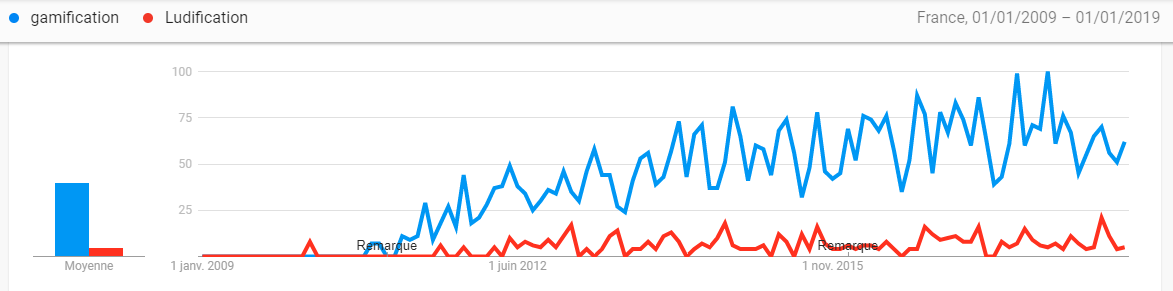
\includegraphics[width=\linewidth]{Images/trends_gamification.png}
    \caption{Évolution de l'intérêt pour la gamification/ludification sur le moteur de recherche Google}
    \source{\cite{gamif-trends}}
    \label{fig:trends}
\end{figure}

\subsection{Données relatives à l'enseignement}
Neuf des articles étudiés ici sont relatifs à l'éducation et à l'apprentissage en général. Comme la majorité des articles traités par Mme Koivisto et MM. Hamari et Sarsa~\cite{gamif-review}, ils font ressortir l’efficacité de la gamification dans le domaine où elle est mise en place. Il est cependant soulevé que l'efficacité finale est variable, bien que globalement positive, et dépend en grande partie de la motivation préexistante des participants pour l’activité proposée. Les mécaniques de jeu mises en place jouent également un rôle et peuvent influencer les résultats. \par 

Il ressort également que dans le domaine de l’enseignement, on constate une amélioration de la motivation, de l‘implication et de la satisfaction des apprenants. En contrepartie, il apparaît également une augmentation de la compétitivité, des risques de mauvaise évaluation de la difficulté d’une tâche et d’erreurs de conception. \par

L'étude pointe cependant que certaines différences de méthodologie et d'échantillonage dans les groupes étudiés peuvent limiter certaines conclusions des auteurs. Ils relèvent notamment certains groupes qu'ils estiment de petite taille ($N=20$ par exemple), sans groupe de contrôle ou sur des durées qui leur semblent courtes. Les résultats sont essentiellement issus des retours directs des participants et sont majoritairement liés à leur comportement durant ces expériences. Enfin, il aurait fallu pour eux que tous les types de motivations possibles soient évalués dans une même étude, ainsi que tous les résultats comportementaux et psychologiques.
